\documentclass[10pt, a4paper]{article}

% DO NOT add \usepackage commands here.  Place any custom commands
% into your SV work files.  Anything in the template directory is
% likely to be overwritten!

\usepackage{fancyhdr}

\usepackage{lastpage}       % ``n of m'' page numbering
\usepackage{lscape}         % Makes landscape easier

\usepackage{verbatim}       % Verbatim blocks
\usepackage{listings}       % Source code listings
\usepackage{graphicx}
\usepackage{float}
\usepackage{epsfig}         % Embed encapsulated postscript
\usepackage{array}          % Array environment
\usepackage{qrcode}         % QR codes
\usepackage{enumitem}       % Required by Tom Johnson's exam question header

\usepackage{hhline}         % Horizontal lines in tables
\usepackage{siunitx}        % Correct spacing of units
\usepackage{amsmath}        % American Mathematical Society
\usepackage{amssymb}        % Maths symbols
\usepackage{amsthm}         % Theorems

\usepackage{ifthen}         % Conditional processing in tex

\usepackage[top=3cm,
            bottom=3cm,
            inner=2cm,
            outer=5cm]{geometry}

% PDF metadata + URL formatting
\usepackage[
            pdfauthor={\studentname},
            pdftitle={\svcourse, SV \svnumber},
            pdfsubject={},
            pdfkeywords={9d2547b00aba40b58fa0378774f72ee6},
            pdfproducer={},
            pdfcreator={},
            hidelinks]{hyperref}

\renewcommand{\headrulewidth}{0.4pt}
\renewcommand{\footrulewidth}{0.4pt}
\fancyheadoffset[LO,LE,RO,RE]{0pt}
\fancyfootoffset[LO,LE,RO,RE]{0pt}
\pagestyle{fancy}
\fancyhead{}
\fancyhead[LO,RE]{{\bfseries \studentname}\\\studentemail}
\fancyhead[RO,LE]{{\bfseries \svcourse, SV~\svnumber}\\\svdate\ \svtime, \svvenue}
\fancyfoot{}
\fancyfoot[LO,RE]{For: \svrname}
\fancyfoot[RO,LE]{\today\hspace{1cm}\thepage\ / \pageref{LastPage}}
\fancyfoot[C]{\qrcode[height=0.8cm]{\svuploadkey}}
\setlength{\headheight}{22.55pt}


\ifthenelse{\equal{\jkfside}{oneside}}{

 \ifthenelse{\equal{\jkfhanded}{left}}{
  % 1. Left-handed marker, one-sided printing or e-marking, use oneside and...
  \evensidemargin=\oddsidemargin
  \oddsidemargin=73pt
  \setlength{\marginparwidth}{111pt}
  \setlength{\marginparsep}{-\marginparsep}
  \addtolength{\marginparsep}{-\textwidth}
  \addtolength{\marginparsep}{-\marginparwidth}
 }{
  % 2. Right-handed marker, one-sided printing or e-marking, use oneside.
  \setlength{\marginparwidth}{111pt}
 }

}{
 % 3. Alternating margins, two-sided printing, use twoside.
}


\setlength{\parindent}{0em}
\addtolength{\parskip}{1ex}

% Exam question headings, labels and sensible layout (courtesy of Tom Johnson)
\setlist{parsep=\parskip, listparindent=\parindent}
\newcommand{\examhead}[3]{\section{#1 Paper #2 Question #3}}
\newenvironment{examquestion}[3]{
\examhead{#1}{#2}{#3}\setlist[enumerate, 1]{label=(\alph*)}\setlist[enumerate, 2]{label=(\roman*)}
\marginpar{\href{https://www.cl.cam.ac.uk/teaching/exams/pastpapers/y#1p#2q#3.pdf}{\qrcode{https://www.cl.cam.ac.uk/teaching/exams/pastpapers/y#1p#2q#3.pdf}}}
\marginpar{\footnotesize \href{https://www.cl.cam.ac.uk/teaching/exams/pastpapers/y#1p#2q#3.pdf}{https://www.cl.cam.ac.uk/\\teaching/exams/pastpapers/\\y#1p#2q#3.pdf}}
}{}


\begin{document}

% 15:51

\begin{enumerate}[label=(\alph*)]

\item 

Let $A$ be the transition matrix. $a_{ij}$ is the probability that the next state will be state $j$ given that 
the current state is state $i$.

$A$ is a $5\times5$ matrix (since there are three hidden states and a start and end state).

\[
A = 
\begin{pmatrix}
a_{SS} & a_{SF} & a_{SL_1} & a_{SL_2} & a_{SE} \\
a_{FS} & a_{FF} & a_{FL_1} & a_{FL_2} & a_{FE} \\
a_{L_1S} & a_{L_1F} & a_{L_1L_1} & a_{L_1L_2} & a_{L_1E} \\
a_{L_2S} & a_{L_2F} & a_{L_2L_1} & a_{L_1L_2} & a_{L_2E} \\
a_{ES} & a_{EF} & a_{EL_1} & a_{EL_2} & a_{EE} \\
\end{pmatrix}
\]

We can estimate $a_{ij}$ by the formula:
\[
a_{ij} = \frac{\mathit{Count}(i \rightarrow j)}{\mathit{Count}(i)}
\]

The sum of each row in the transiiton matrix is 1 since every state must transition to some state.

By definition, since $S$ is the start state and only occurs at the start of a sequence, the probability of 
a state transitioning to $S = 0$ for any state. Note also that the probability of $E$ transitioning into any 
other state is also zero (the HMM would terminate when the state became $E$ but for the purposes of this question 
I will mark the probability of $E$ transitioning to $E$ as 1 and any other state as 0).

Let $B$ be the emission matrix. $b_{ij}$ is the probability that hidden state $i$ emits symbol $j$. 

$B$ is a $5 \times 8$ matrix -- since there are 5 hidden states (including the two special states for start 
and end) and 8 symbols in the emission alphabet (one for each dice roll and two special ones [$k_s$ and $k_e$] for start and end).

\[
B = 
\begin{pmatrix}
b_{Sk_s} & b_{S1} & b_{S2} & b_{S3} & b_{S4} & b_{S5} & b_{S6} & b_{Sk_e} \\
b_{Fk_s} & b_{F1} & b_{F2} & b_{F3} & b_{F4} & b_{F5} & b_{F6} & b_{Fk_e} \\
b_{L_1k_s} & b_{L_11} & b_{L_12} & b_{L_1L_3} & b_{L_14} & b_{L_15} & b_{L_16} & b_{L_1k_e}\\
b_{L_2k_s} & b_{L_21} & b_{L_22} & b_{L_13} & b_{L_24} & b_{L_25} & b_{L_26} * b_{L_2k_e}\\
b_{Ek_s} & b_{E1} & b_{E2} & b_{E3} & b_{E4} & b_{E5} & b_{E6} & b_{Ek_e}\\
\end{pmatrix}
\]

We can estimate $b_{ij}$ by the formula:
\[
b_{ij} = \frac{\mathit{Count}(i, j)}{\mathit{Count}(i)}
\]

Note that since by definition, $k_s$ is the state emitted by the start state; $b_{Si}$ for $i \neq k_s$ will be 
0 and $b_{Sk_s} = 1$. The same statement holds for the end state $E$ and the end symbol $k_e$.

The sum of each row in the emission matrix sums to one -- since every state is guaranteed to emit some symbol.

\item 

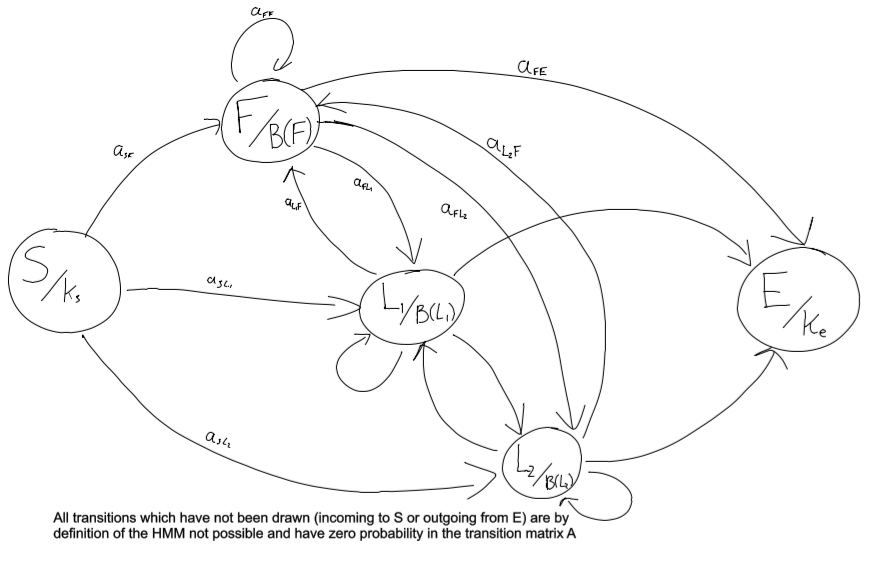
\includepdf{mlrwd_sample_diagram.png}

\item 

\begin{enumerate}[label=(\alph*)]

\item The probability $a_{FL_2}$ is equal to zero.

Setting this probability to zero means that it is impossible for the HMM to model a switch directly from 
$F$ to $L_2$. The HMM would now model this.

\item For all hidden states $s$, $s \neq F \Longleftrightarrow a_{sE} = 0$.

IE the probability of transitioning from any state which is not $F$ to the end state $E$ is zero.

This model will ensure that every sequence ends on $F$ -- as the croupier does.

\item $a_{L_2L_2} = 0$

IE the probability of transitioning from $L_2$ to $L_2$ is zero. So the HMM cannot model it happening 
and the HMM now models the new behavior appropriately.

We would have to maintain the invariant that the outgoing probabilities of $L_2$ sum to 1.

\item This can't be modelled by the HMM \dag. By definition of the HMM, the next state is only dependent on the 
previous state -- and not on the emissions. So the emission of the previous state can have no impact on the 
next state. So the HMM cannot model this behavior.

\dag with the exception of the case where one dice $d$ always rolls a 6 -- in this case $a_{dd} = 0$.

\end{enumerate}

\end{enumerate}

\end{document}
